\documentclass[12pt,a4paper]{article}
\usepackage{graphicx}
\usepackage{wrapfig}
\usepackage{textcomp}

\title{Praktikum Physik - Wechselstrom}
\author{Simon Marti, Patricia Schwab, Mirco Kocher}
\date{27.04.2012}


\begin{document}
\maketitle

\section*{Ziel}
Durch das Verh\"altnises der Spannungsamplituden von verschiedenen Frequenzen soll die Impedanz berechnet werden.
Ausserdem soll f\"ur kleine Frequenzen die Phasenverschiebung zwischen Strom und Spannung bestimmt werden.


\section*{Motivation}
Dieser Versuch soll dazu beitragen, Wechselstromschaltungen und die Funktionsweise des Kathodenstrahloszilloskop ("KO") zu verstehen.
Das KO hat sich zur Darstellung und Analyse von Wechselstr\"omen als \"ausserst hilfreich erwiesen.
Viele Anwedungen beruhen auf den besonderen Eigenschaften des Wechselstroms, insbesondere im Zusammenhang mit den elektronischen Bauteilen Kondensator und Spule.


\section*{Theorie}
Die Kreisfrequenz $\omega$ l\"asst sich mit der Frequenz $f$ folgendermassen bestimmen
\begin{equation}
\omega = 2\pi f
\end{equation}
Die Impedanz eines Widerstandes $R$ und eines Kondensators $C$ ("RC-Glied") $Z_{RC}$ kann durch die sinusf\"ormige Eingangsspannung $U_E$, die Ausgangsspannung $U_A$ und der Impedanz des Kondensators $Z_C$ bzw. der Kapazit\"at $C$ berechnet werden
\begin{equation}
|Z_{RC}| = \left| \frac{U_E}{U_A} \right| \cdot |Z_C| = \left| \frac{U_E}{U_A} \right| \frac{1}{\omega C}
\end{equation}
Die Formel f\"ur das Spannungsverh\"altnis der Ausgangsspannung $U_A$ zur Eingangsspannung $U_E$ eines Tiefpasses mit der imagin\"aren Zahl $j$ ist
\begin{equation}
\left| \frac{U_A}{U_E} \right|= \left| \frac{\frac{1}{j\omega C}}{R + \frac{1}{j\omega C}}\right| = \frac{1}{\sqrt{1+(\omega RC)^2}}
\end{equation}
Die Phasenverschiebung $\varphi$  eines Hochpasses ist gegeben durch
\begin{equation}
tan(\varphi) = \frac{1}{\omega R C}
\end{equation}

\section*{Aufgabe I}
\begin{eqnarray*}
Z_L & = & j \omega L \\
Z_R & = & R \\
Z_{Total} & = & \left( \frac{1}{j \omega L} + \frac{1}{R} \right) ^{-1} \\
& = & \frac{j \omega L R}{R + j \omega L}
\end{eqnarray*}


\section*{Aufgabe II}
\subsection*{Aufbau und Ablauf}
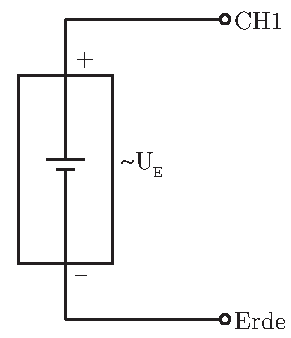
\includegraphics[height=5cm]{illustration2.pdf}

Das Oszilloskop wird direkt an den Frequenzgenerator angeschlossen.

\subsection*{Diskussion}
Damit sich auf dem Bildschirm des KO ein stehendes Bild ergibt, muss die Zeitablenkung immer beim selben Wert der Signalspannung beginnen. Dies wird durch das Triggerniveau und die Triggerflanke gesteuert.
Aufgrund der Sinusform ist das Bild am klarsten, wenn das Triggerniveau in der Mitte der Signalspannung liegt. Je weiter weg es vom Zentrum verschoben wird, desto diffuser ist das angezeigte Bild und es ist unbrauchbar, wenn das Triggerniveau h\"oher als die Signalspannung angelegt ist.
Die ver\"anderung der Triggerflanke f\"uhrt lediglich zu einer Verschiebung der Signalspannung um eine halbe Periode.


\section*{Aufgabe III}
\subsection*{Aufbau und Ablauf}
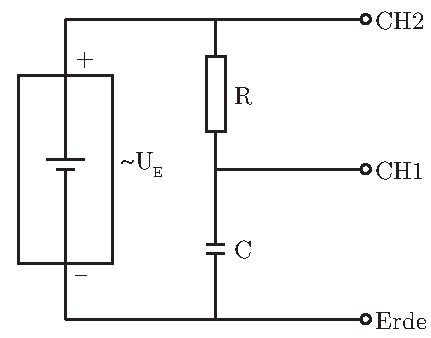
\includegraphics[height=5cm]{illustration3.pdf}

\noindent
Ein RC-Schaltung wird gem\"ass Schaltschema aufgebaut und das Oszilloskop sowohl \"uber dem Widerstand wie auch dem Frequenzgenerator angeschlossen. F\"ur verschiedene Frequenzen $f$ wurden die Spannungsamptlituden $U_E$ und $U_A$ bestimmt.

\subsection*{Rohdaten} 
\begin{tabular}{|r|r|r|}
\hline
$f$ [Hz]&$U_E$ [V]&$U_A$ [V]\\
\hline
$137.0 \pm 0.5$&$3.50 \pm 0.1$&$461\cdot 10^{-3} \pm 10^{-3}$\\
$733 \pm 1$&$3.40 \pm 0$&$196\cdot 10^{-3} \pm 0$\\
$35.46 \pm 0.03$&$3.41 \pm 0.01$&$1.42 \pm 0.01$\\
$4.080\cdot 10^{3} \pm 5$&$3.40 \pm 0.01$&$180\cdot 10^{-3} \pm 2\cdot 10^{-3}$\\
$4.120\cdot 10^{3} \pm 500$&$3.40 \pm 0.01$&$184\cdot 10^{-3} \pm 10^{-3}$\\
$480.0\cdot 10^{3} \pm 1000$&$3.20 \pm 0.01$&$177\cdot 10^{-3} \pm 10^{-3}$\\
$990\cdot 10^{3} \pm 8000$&$2.72 \pm 0.02$&$163\cdot 10^{-3} \pm 10^{-3}$\\
\hline
\end{tabular}

\subsection*{Auswertung}
TODO

\subsection*{Diskussion}
TODO (Mirco)


\section*{Aufgabe IV}
\subsection*{Aufbau und Ablauf}
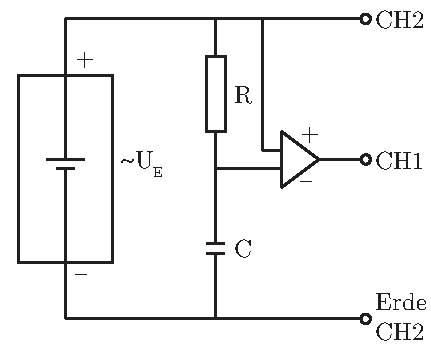
\includegraphics[height=5cm]{illustration4.pdf}

\noindent
In die Schaltung aus Aufgabe 3 wied gem\"ass Schaltschema ein Differenzverst\"arker eingebaut. F\"ur mehrere Frequenzen $f$ wird die Phasenverschiebung $\varphi$ gemessen.

\subsection*{Rohdaten}
\begin{tabular}{|r|r|}
\hline
$f$ [Hz]&$\varphi$ [s]\\
\hline
$58.7 \pm 0.07$&$720\cdot 10^{-6} \pm 50\cdot 10^{-6}$\\
$23.50 \pm 0.03$&$4.6\cdot 10^{-3} \pm 0.1\cdot 10^{-3}$\\
$607 \pm 2$&$18\cdot 10^{-6} \pm 0.5\cdot 10^{-6}$\\
$296 \pm 0.2$&$53.60\cdot 10^{-6} \pm 1\cdot 10^{-6}$\\
$3.425\cdot 10^{3} \pm 50$&$1.580\cdot 10^{-6} \pm 0.1\cdot 10^{-6}$\\
$7.215\cdot 10^{3} \pm 1$&$360\cdot 10^{-9} \pm 30\cdot 10^{-9}$\\
$36.64\cdot 10^{3} \pm 0$&$394\cdot 10^{-9} \pm 15\cdot 10^{-9}$\\
$58.24\cdot 10^{3} \pm 10$&$776\cdot 10^{-9} \pm 6\cdot 10^{-9}$\\
$177.8\cdot 10^{3} \pm 300$&$1.36\cdot 10^{-6} \pm 0$\\
$217.9\cdot 10^{3} \pm 500$&$1.24\cdot 10^{-6} \pm 0$\\
\hline
\end{tabular}

\subsection*{Auswertung}
TODO

\subsection*{Diskussion}
TODO (Mirco)

\end{document}